%% BioMed_Central_Tex_Template_v1.06
%%                                      %
%  bmc_article.tex            ver: 1.06 %
%                                       %

%%IMPORTANT: do not delete the first line of this template
%%It must be present to enable the BMC Submission system to
%%recognise this template!!

%%%%%%%%%%%%%%%%%%%%%%%%%%%%%%%%%%%%%%%%%
%%                                     %%
%%  LaTeX template for BioMed Central  %%
%%     journal article submissions     %%
%%                                     %%
%%          <8 June 2012>              %%
%%                                     %%
%%                                     %%
%%%%%%%%%%%%%%%%%%%%%%%%%%%%%%%%%%%%%%%%%


%%%%%%%%%%%%%%%%%%%%%%%%%%%%%%%%%%%%%%%%%%%%%%%%%%%%%%%%%%%%%%%%%%%%%
%%                                                                 %%
%% For instructions on how to fill out this Tex template           %%
%% document please refer to Readme.html and the instructions for   %%
%% authors page on the biomed central website                      %%
%% http://www.biomedcentral.com/info/authors/                      %%
%%                                                                 %%
%% Please do not use \input{...} to include other tex files.       %%
%% Submit your LaTeX manuscript as one .tex document.              %%
%%                                                                 %%
%% All additional figures and files should be attached             %%
%% separately and not embedded in the \TeX\ document itself.       %%
%%                                                                 %%
%% BioMed Central currently use the MikTex distribution of         %%
%% TeX for Windows) of TeX and LaTeX.  This is available from      %%
%% http://www.miktex.org                                           %%
%%                                                                 %%
%%%%%%%%%%%%%%%%%%%%%%%%%%%%%%%%%%%%%%%%%%%%%%%%%%%%%%%%%%%%%%%%%%%%%

%%% additional documentclass options:
%  [doublespacing]
%  [linenumbers]   - put the line numbers on margins

%%% loading packages, author definitions

%\documentclass[twocolumn]{bmcart}% uncomment this for twocolumn layout and comment line below
\documentclass{bmcart}

%%% Load packages
%\usepackage{amsthm,amsmath}
%\RequirePackage{natbib}
%\RequirePackage[authoryear]{natbib}% uncomment this for author-year bibliography
%\RequirePackage{hyperref}
\usepackage[utf8]{inputenc} %unicode support
%\usepackage[applemac]{inputenc} %applemac support if unicode package fails
%\usepackage[latin1]{inputenc} %UNIX support if unicode package fails

%%%%%%%%%%%%%%%%%%%%%%%%%%%%%%%%%%%%%%%%%%%%%%%%%
%%                                             %%
%%  If you wish to display your graphics for   %%
%%  your own use using includegraphic or       %%
%%  includegraphics, then comment out the      %%
%%  following two lines of code.               %%
%%  NB: These line *must* be included when     %%
%%  submitting to BMC.                         %%
%%  All figure files must be submitted as      %%
%%  separate graphics through the BMC          %%
%%  submission process, not included in the    %%
%%  submitted article.                         %%
%%                                             %%
%%%%%%%%%%%%%%%%%%%%%%%%%%%%%%%%%%%%%%%%%%%%%%%%%

\usepackage{todonotes}
\usepackage{graphicx}
\usepackage{amsmath}
\usepackage{url}
\usepackage{subcaption}
%\def\includegraphic{}
%\def\includegraphics{}



%%% Put your definitions there:
\startlocaldefs
\endlocaldefs


%%% Begin ...
\begin{document}
	
	%%% Start of article front matter
	\begin{frontmatter}
		
		\begin{fmbox}
			\dochead{Methodology}
			
			%%%%%%%%%%%%%%%%%%%%%%%%%%%%%%%%%%%%%%%%%%%%%%
			%%                                          %%
			%% Enter the title of your article here     %%
			%%                                          %%
			%%%%%%%%%%%%%%%%%%%%%%%%%%%%%%%%%%%%%%%%%%%%%%
			
			\title{Statistical Stopping Criteria for Active Learning in Systematic Review Screening}
			
			%%%%%%%%%%%%%%%%%%%%%%%%%%%%%%%%%%%%%%%%%%%%%%
			%%                                          %%
			%% Enter the authors here                   %%
			%%                                          %%
			%% Specify information, if available,       %%
			%% in the form:                             %%
			%%   <key>={<id1>,<id2>}                    %%
			%%   <key>=                                 %%
			%% Comment or delete the keys which are     %%
			%% not used. Repeat \author command as much %%
			%% as required.                             %%
			%%                                          %%
			%%%%%%%%%%%%%%%%%%%%%%%%%%%%%%%%%%%%%%%%%%%%%%
			
			\author[
			addressref={aff1,aff2},                   % id's of addresses, e.g. {aff1,aff2}
			corref={aff1},                       % id of corresponding address, if any
			%noteref={n1},                        % id's of article notes, if any
			email={callaghan@mcc-berlin.net}   % email address
			]{\inits{MW}\fnm{Max W} \snm{Callaghan}}
			\author[
			addressref={aff1},
			email={mueller-hansen@mcc-berlin.net}
			]{\inits{FMH}\fnm{Finn} \snm{M\"{u}ller-Hansen}}
			
			%%%%%%%%%%%%%%%%%%%%%%%%%%%%%%%%%%%%%%%%%%%%%%
			%%                                          %%
			%% Enter the authors' addresses here        %%
			%%                                          %%
			%% Repeat \address commands as much as      %%
			%% required.                                %%
			%%                                          %%
			%%%%%%%%%%%%%%%%%%%%%%%%%%%%%%%%%%%%%%%%%%%%%%
			
			\address[id=aff1]{%                           % unique id
				\orgname{Mercator Research Institute on Global Commons and Climate Change}, % university, etc
				\street{Torgauer Straße},                     %
				\postcode{10829}                                % post or zip code
				\city{Berlin},                              % city
				\cny{Germany}                                    % country
			}
			\address[id=aff2]{%
				\orgname{Priestley International Centre for Climate, University of Leeds, Leeds },
				%\street{Dsternbrooker Weg 20},
				\postcode{LS2 9JT}
				\city{Leeds},
				\cny{United Kingdom}
			}
			
			%%%%%%%%%%%%%%%%%%%%%%%%%%%%%%%%%%%%%%%%%%%%%%
			%%                                          %%
			%% Enter short notes here                   %%
			%%                                          %%
			%% Short notes will be after addresses      %%
			%% on first page.                           %%
			%%                                          %%
			%%%%%%%%%%%%%%%%%%%%%%%%%%%%%%%%%%%%%%%%%%%%%%
			
			\begin{artnotes}
				%\note{Sample of title note}     % note to the article
				%\note[id=n1]{Equal contributor} % note, connected to author
			\end{artnotes}
			
		\end{fmbox}% comment this for two column layout
		
		%%%%%%%%%%%%%%%%%%%%%%%%%%%%%%%%%%%%%%%%%%%%%%
		%%                                          %%
		%% The Abstract begins here                 %%
		%%                                          %%
		%% Please refer to the Instructions for     %%
		%% authors on http://www.biomedcentral.com  %%
		%% and include the section headings         %%
		%% accordingly for your article type.       %%
		%%                                          %%
		%%%%%%%%%%%%%%%%%%%%%%%%%%%%%%%%%%%%%%%%%%%%%%
		
		\begin{abstractbox}
			
			\begin{abstract} % abstract
				%\parttitle{First part title} %if any
				Active learning for systematic review screening promises to reduce the human effort required to identify relevant documents for a systematic review. 
				Machines and humans  work together, with the human providing training data, and the machine optimising the documents a human screens, so that they can identify all relevant documents after viewing only a fraction of the total documents. 
				However, current approaches lack robust stopping criteria, so that reviewers do not know when they have seen all or a certain proportion of relevant documents. This means that such systems are hard to implement in live reviews. 
				This paper introduces a workflow for working with robust and flexible statistical stopping criteria, that offer real work reductions on the basis of a given confidence level of reaching a given recall.
				The stopping criteria is shown on test datasets to achieve a reliable level of recall, while still providing consistent work reductions, while other methods proposed are shown to provide inconsistent recall and work reductions across datasets.
				
			\end{abstract}
			
			%%%%%%%%%%%%%%%%%%%%%%%%%%%%%%%%%%%%%%%%%%%%%%
			%%                                          %%
			%% The keywords begin here                  %%
			%%                                          %%
			%% Put each keyword in separate \kwd{}.     %%
			%%                                          %%
			%%%%%%%%%%%%%%%%%%%%%%%%%%%%%%%%%%%%%%%%%%%%%%
			
			\begin{keyword}
				\kwd{Systematic Review}
				\kwd{Machine Learning}
				\kwd{Active Learning}
				\kwd{Stopping Criteria}
			\end{keyword}
			
			% MSC classifications codes, if any
			%\begin{keyword}[class=AMS]
			%\kwd[Primary ]{}
			%\kwd{}
			%\kwd[; secondary ]{}
			%\end{keyword}
			
		\end{abstractbox}
		%
		%\end{fmbox}% uncomment this for twcolumn layout
		
	\end{frontmatter}

%%%%%%%%%%%%%%%%%%%%%%%%%%%%%%%%%%%%%%%%%%%%%%
%%                                          %%
%% The Main Body begins here                %%
%%                                          %%
%% Please refer to the instructions for     %%
%% authors on:                              %%
%% http://www.biomedcentral.com/info/authors%%
%% and include the section headings         %%
%% accordingly for your article type.       %%
%%                                          %%
%% See the Results and Discussion section   %%
%% for details on how to create sub-sections%%
%%                                          %%
%% use \cite{...} to cite references        %%
%%  \cite{koon} and                         %%
%%  \cite{oreg,khar,zvai,xjon,schn,pond}    %%
%%  \nocite{smith,marg,hunn,advi,koha,mouse}%%
%%                                          %%
%%%%%%%%%%%%%%%%%%%%%%%%%%%%%%%%%%%%%%%%%%%%%%

%%%%%%%%%%%%%%%%%%%%%%%%% start of article main body
% <put your article body there>

%%%%%%%%%%%%%%%%
%% Background %%
%%
	
	%%%%%%%%%%%%%%%%%%%%%%%%
	%% Introduction
	\section*{Background}
	
	Machine learning for evidence synthesis is a growing field, where machine learning enabled interventions are introduced at various points in the workflow, in order to reduce the human effort required to produce systematic reviews and other forms of evidence synthesis.
	A major strand of the literature works on screening - the identification of relevant documents in a set of documents whose relevance is uncertain \cite{OMara-Eves2015}. 
	For this task, several papers have developed or evaluated active learning. 
	
	Active learning is an iterative process where documents screened by humans are used to train a machine learning model to predict the relevance of unseen papers \cite{Settles2009}.
	The most relevant studies are passed back to the human and rated, generating more labels to feed back to the machine. 
	By prioritising those studies most likely to be relevant, a human reviewer most often identifies all relevant studies - or a given proportion of relevant studies (recall) - before having seen all the documents in the corpus. 
	The proportion of documents not yet seen by the human when they reach the given recall threshold are referred to as the work saved.
	
	In live review settings, however, the recall remains unknown until all documents have been screened. 
	In order for work to really be saved, reviewers have to stop screening while uncertain about the recall. This is particularly problematic in systematic reviews because low recall increases the risk of publication bias %\cite{Lefebrve in Cochrane}
	The lack of appropriate stopping criteria has therefore been identified as a research gap \cite{bannach-brown2019}, although some approaches have been suggested. These fall into the following categories
	\begin{itemize}
		\item \textbf{Sampling criteria:} Reviewers estimate the number of relevant documents by taking a random sample at the start of the process. They stop when this number, or a given proportion of it, has been reached \cite{Shemilt2014}
		\item \textbf{Heuristics:} Reviewers stop when a given number of irrelevant articles are seen in a row \cite{Przybya2018}. 
		\item \textbf{Pragmatic criteria:} Reviewers stop when they run out of time \cite{miwa2014}. 
	\end{itemize}
	
	We show in this paper how the first two criteria are inadequate.
	We argue that the inadequacy lies in the unreliability - particularly across different domains, or datasets with different properties \todo{ref on cross-domain reliability} - both of the work saved and the recall achieved. Not achieving the desired level of recall is a particular challenge for systematic review screening. In systematic reviews, the larger the proportion of the relevant literature is not considered, the greater the risk of publication bias \todo{ref cochrane handbook}. 
	Without the reliable or reportable achievement of a desired level of recall, AL systems in live reviews remain challenging.
	
	This study proposes a system for estimating the recall based on random sampling of remaining documents. 
	We draw on the literature on binomial distributions \cite{Brown2001}, to illustrate how AL users can predefine a threshold in terms of uncertainty and recall, and use this to transparently save work with machine learning, while making a statement like ``There is a <5\% chance that we achieve a recall under 95\%''.
	
	The information retrieval literature discusses similar stopping criteria for ranking algorithms like BM25 and variants \cite{DiNunzio2018, Yu2019}. However, the estimators they use to determine the recall rely on the specific ranking functions and depend on their search input. Therefore, the quality of the estimation depends on the adequacy of the model. Our approach, on the contrary, is independent of model choice or model performance. 
	
	We evaluate this stopping criteria on real-world systematic review datasets on which active learning systems have previously been tested.
	
	\section*{Methods}
	
	\subsection*{Existing Stopping Criteria for Active Learning}
	
	We start by explaining the sampling and heuristic based stopping criteria before showing with toy data how the criteria fall short. 
	Then we introduce our own suggested stopping criteria, and show its benefits with toy data, before testing all criteria on real world datasets.
	
	\subsubsection*{Sampling Based Stopping Criteria}
	
	The stopping criterion suggested by \cite{Shemilt2014} involves establishing the Baseline Inclusion Rate (BIR), by taking a random sample at the beginning of screening. 
	This is used to estimate the number of relevant documents in the whole dataset. 
	Reviewers continue to screen until this number, or a proportion of it corresponding to the desired level of recall, is reached.
	

	
	However, the estimation of the BIR fails to take into account the sampling uncertainty. 
	Figure \ref{bir-sampling}.a shows for 50 random samples of 2,000 documents from 20,000 documents (where 5\% of documents are relevant), the predicted number of documents after each document drawn. 
	Depending on the luck of the draw, one might estimate the true number of documents as being
	\begin{itemize}
		\item much higher than the true value, meaning that the stopping criterion would never be reached - and no work could be saved
		\item much lower than the true value, meaning that the stopping criterion would be reached before the desired level of recall was actually achieved
	\end{itemize}
	
	We can estimate the uncertainty of a binomial outcome using an Agresti-Coull confidence interval (which has been shown to be conservative at levels near 0 \todo{this is less relevant here, go back to literature and see if another is better} \cite{Brown2001}). 
	Figure \ref{bir-sampling}.b shows the 95\% confidence interval (brown) and its upper bound (green) in the same set of random draws. 
	Where the green line is above the above the lower (upper) grey line, identification of 100\% (95\%) of the estimated number of studies would be impossible, and no work would be saved.
	
	Figure \ref{bir-variation} explores different scenarios of true relevance and probability thresholds, showing that the higher the true proportion of relevant documents, the fewer documents one would have to sample to make the identification of a given fraction (the true number of relevant results divided by the upper estimate) possible. 
	\todo{Why does it behave like this, is there a theoretical maximum for each? something to do with absolute values? a Bug? Is uncertainty a function of being near to 0?} 
	Even with a relatively high proportion of relevant documents, and a sample of 500, all relevant documents would have to be identified to have a 95\% likelihood of achieving 95\% recall. 
	With low proportions of relevant documents, only an 80\% recall can be estimated with confidence, even after a sample of 2000, and subsequently identifying all relevant documents. 
	N.B, these results ignore the random element of sample order, which explains the variation on figure \ref{bir-sampling}. 
	They show upper confidence bounds for accurate estimates of relevance.

	\begin{figure}
	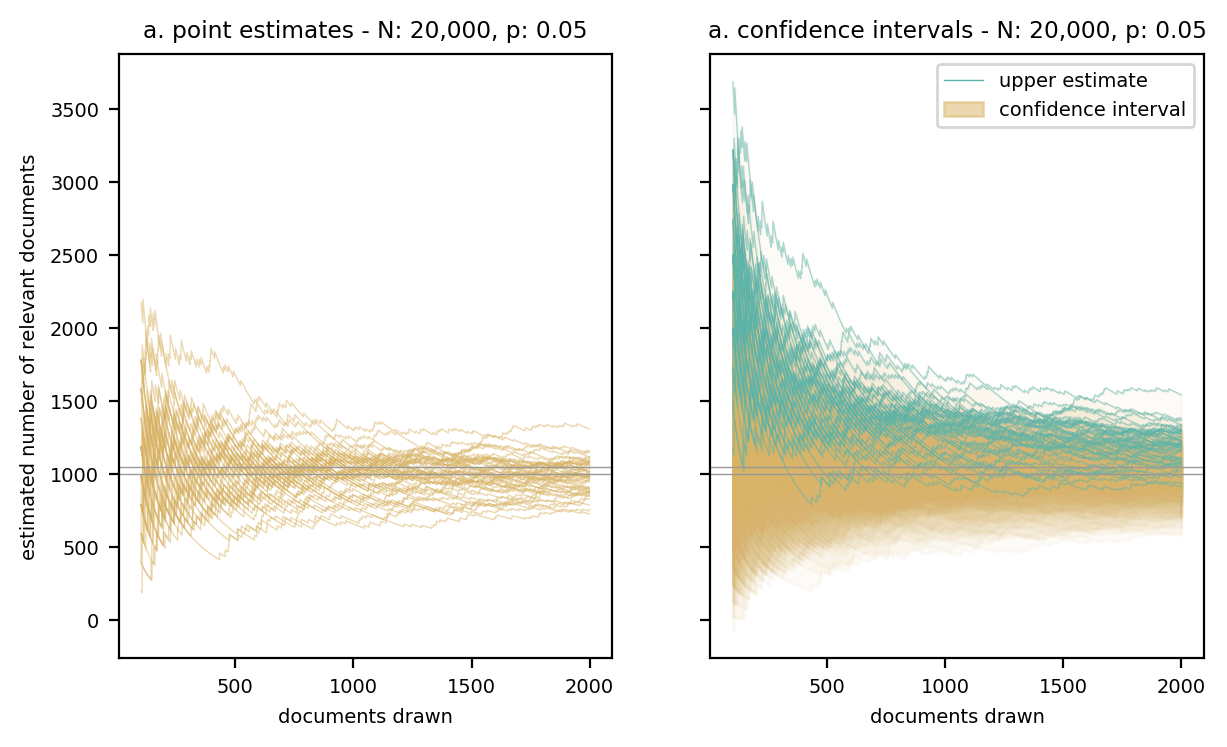
\includegraphics[width=\linewidth]{../images/bir_sampling.png}
	\caption{Uncertainty in estimating the baseline inclusion rate. a. shows the estimated BIR after drawing each document, for 50 random samples of from 20,000 documents, after each document is drawn. b. Shows the 95\% Confidence interval (brown) and the upper bound (green) for each of the same samples. The two lines correspond to 100\% of relevant documents, and $\frac{100}{0.95}$\% of relevant documents.}
	\label{bir-sampling}
\end{figure}

\begin{figure}
	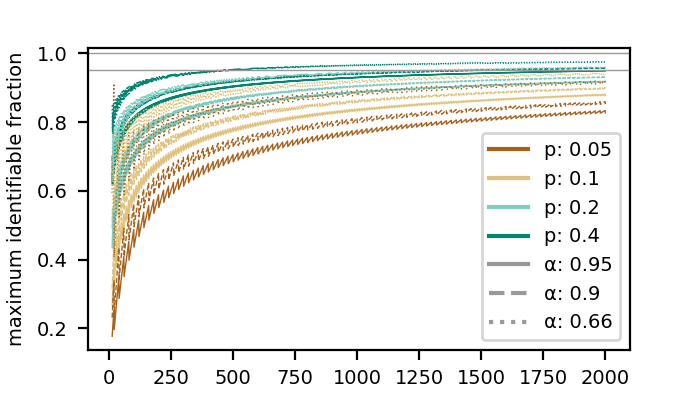
\includegraphics[width=0.5\linewidth]{../images/bir_variation.png}
	\caption{Maximum indentifiable fraction of relevant results under different levels of true relevance $p$ and confidence thresholds $\alpha$. Maximum identifiable fraction is the true number of relevant documents divided by the upper estimate.}
	\label{bir-variation}
\end{figure}

		
\subsubsection*{Heuristic Based Stopping Criteria}

Some studies give the example of heuristic based stopping criteria based on drawing a given number of irrelevant articles in a row \cite{Przybya2018} [+REFS]. 
We take this as a proxy for estimating that the proportion of documents remaining in the unseen documents is low. 
We find this a promising intuition, but argue that 1) it ignores uncertainty, as discussed in relation to the previous method; and 2) it misunderstands the significance of a low proportion of relevant documents in estimating the recall.

Figure \ref{unseen-proportions} illustrates this second point. 
We show two scenarios with identical low proportions of relevant documents (note that estimating a proportion lower than 0.02 with 95\% confidence requires 160 consecutive irrelevant documents)\todo{demonstrate?}. 
Recall is not simply a function of the relevance of unseen documents, but also of the number of unseen documents. 
This also means that where machine learning has performed well (as in the top figure), low proportions of irrelevant documents in those that remain are indicative of lower recall than where ML has performed less well.

\begin{figure}
	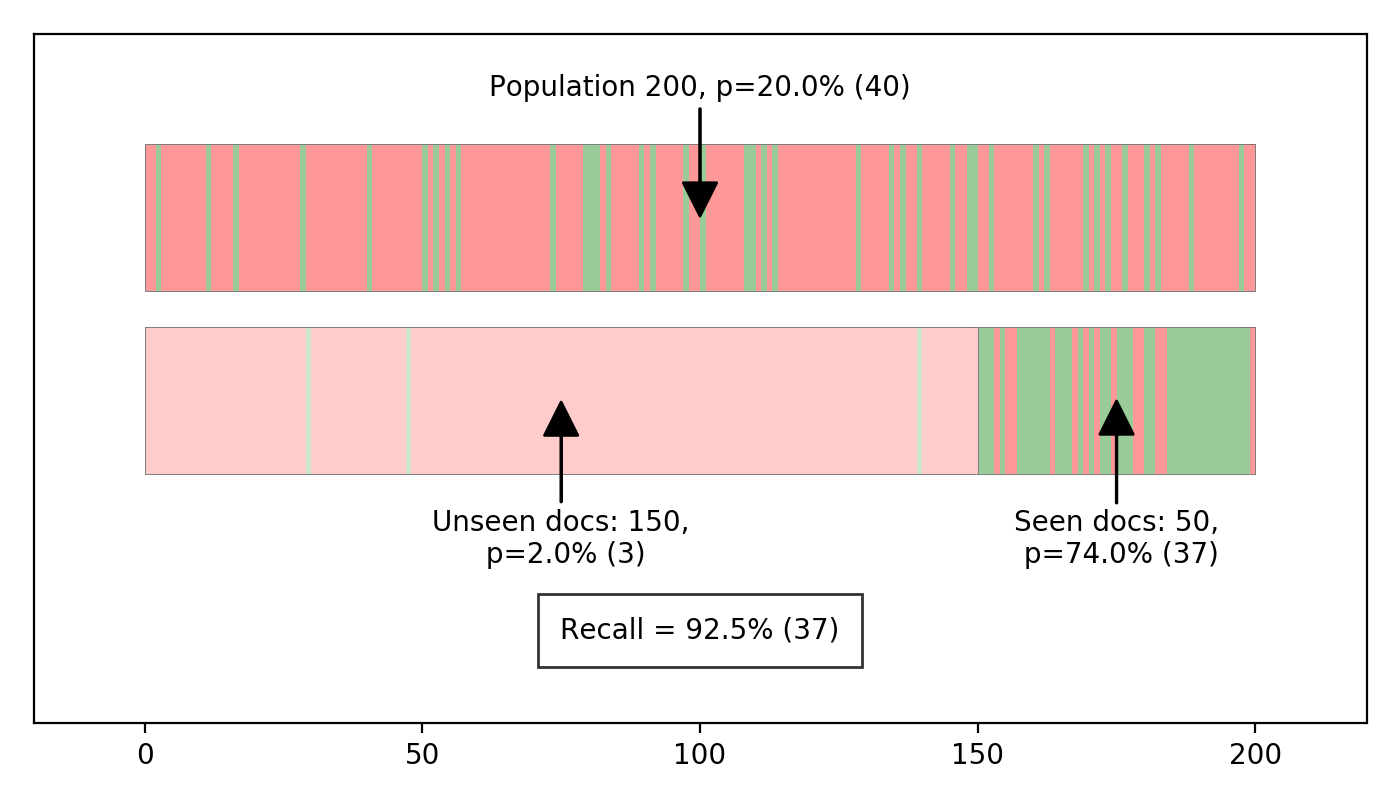
\includegraphics[width=\linewidth]{../images/proportions_1.png}
	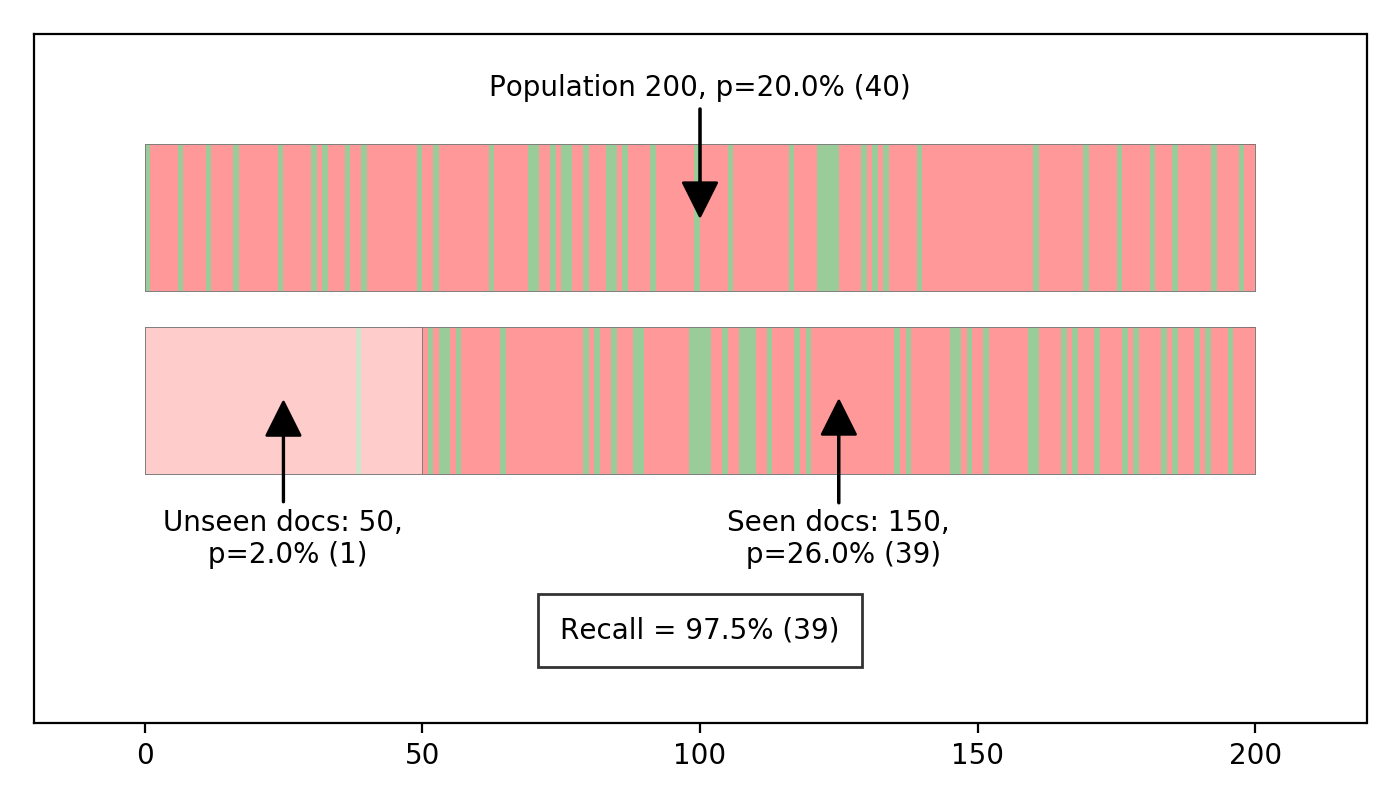
\includegraphics[width=\linewidth]{../images/proportions_2.png}
	\caption{Similar low proportions of relevant documents in unseen documents with different consequences for recall. The top bar shows a random distribution of relevant documents (green) and irrelevant documents (red) at a given proportion of relevance. The bottom bar  shows distributions of relevant and irrelevant documents in hypothetical sets of seen (right) and unseen (left - transparent) documents.}
	\label{unseen-proportions}
\end{figure}

\subsubsection*{Other stopping criteria}

\cite{Wallace2010a} Develop a ``simple, operational stopping criterion'': stopping after half the documents have been screened. Although the criterion worked in their experiment, it is unclear how this could be generalised, and its development depended on knowledge of the true relevance values. 
\cite{Jonnalagadda2013} note that ``the reviewer can elect to end the process of classifying documents at any point, recognizing that stopping before reviewing all documents involves a trade-off of lower recall for reduced workload'', although clearly the reviewer lacks information about probable recall.
\cite{Yu2019} adopt a more complicated stopping criterion \todo{How does it actually work??} which allows the user to target a specific level of recall. However, reviewers are not given the opportunity to specify a confidence level, and for two of the four datasets in which they tested their criteria, the median achieved recall at a stopping criteria targeting 95\% recall was below 95\%. \cite{DiNunzio2018} also present an innovative stopping criteria, but it does not take into account uncertainty, and produces results \textit{near} a target recall threshold. 
These last examples are promising developments, but [are not ready for live reviews because hard to understand/communicate?? do not give uncertainty about reaching a threshold]



\subsection*{A Statistical Stopping Criterion for Active Learning}

	\subsection*{Random Sampling}

	Using the cumulative distribution function of the hypergeometric distribution, we can estimate the probability of observing $k$ or fewer relevant documents after drawing $N$ documents without replacement from a pool of $M$ documents, of which $n$ are relevant.
	
	The probability mass function is defined as,

	\begin{equation}	
		 p(k, M, n, N) = \frac{\binom{n}{k} \binom{M - n}{N - k}} {\binom{M}{N}}	
		 \label{pfunc}
	\end{equation}
	
	After seeing a proportion of the documents in a query, we can set $M$ to the number of documents remaining, and begin drawing documents at random from the remaining unseen documents. After each draw, $k$ is the number of relevant documents seen since sampling began, and $N$ is the number of documents sampled. We can generate a counterfactual $\hat{n}$, corresponding to the largest integer greater than the number of relevant documents seen $\rho$ divided by the recall target $\tau$ minus the relevant documents seen before random sampling began $\hat{\rho}$
	
	\begin{equation}
	\hat{n} = \lceil \frac{\rho}{\tau} - \hat{\rho} \rceil
	\end{equation}
	
	
	Substituting $\hat{n}$ into equation \ref{pfunc}, we can generate the $p$, the probability of observing $k$ or fewer documents if our recall target had been reached. If this is below $1-\alpha$, our confidence level, we can be $\alpha$ confident that our target has been reached.
	
	\subsection*{Pseudo-random sampling}
	In order to decide when to begin a random sample, we employ pseudo-random sampling, where we treat previously screened documents as a random sample. The distribution of relevant documents among previously screened documents is clearly not random, as documents predicted to be relevant are prioritised. It is reasonable to assume, though, that the distribution of relevant documents is greater among previously screened documents than among remaining unseen documents. This would make the following estimates conservative. 
	
	After reviewing each document, $S$ documents are screened, and $U$ documents are yet to be seen. We treat $i = 1 \dots S$ of the previously screened documents as a random sample, and calculate $p$ as before for each sample, taking the minimum across all samples $\dot{p}$. If $\dot{p}$ is less than $1-\frac{\alpha}{2}$, we switch to random sampling. We also calculate $\dot{p}$ for the remaining values as if we had not switched to random sampling and present these in the results below.


	\medskip
	
	\subsection*{Old description}


	Figure \ref{flow} shows a workflow for the approach proposed in this paper. 
	The random sampling occurs at the end of the process, and is used to estimate the number of relevant documents remaining and the total number of relevant documents. 
	The rationale is to limit the uncertainty to a subsection of the dataset: that which has not yet been screened. 
	As reviewers continue to draw random documents, the uncertainty range decreases, and the proportion of the data about which one is uncertain also decreases.
	
	\begin{figure}
		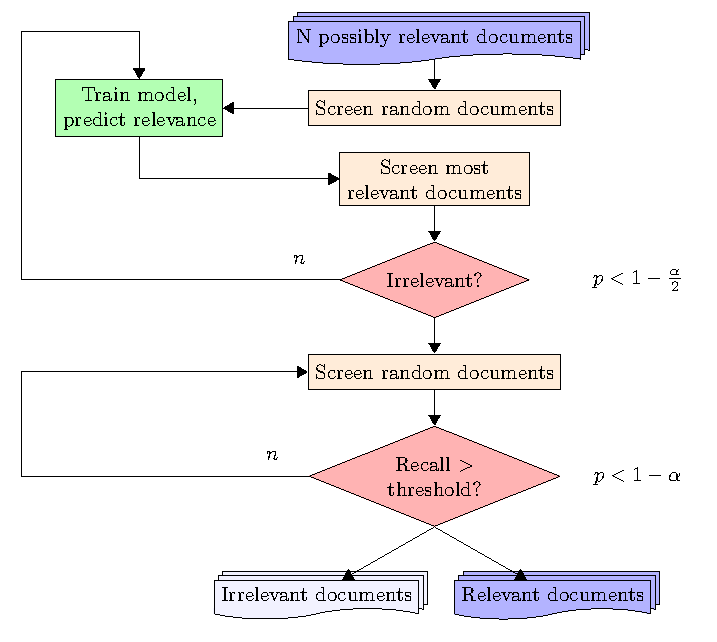
\includegraphics[width=0.5\linewidth]{../images/flow}
		\caption{A workflow for active learning in screening with a statistical stopping criterion}
		\label{flow}
	\end{figure}
	
	\begin{table}
		\begin{tabular}{p{0.15\linewidth} p{0.425\linewidth} p{0.425\linewidth}}
			Parameter & Description & Estimation \\
			\hline
			$ P  $ &  Total number of studies & \textit{Observed} \\
			$ S $ & Number of studies coded by humans & \textit{Observed} \\
			$ U $ & Number of studies not yet coded by humans & \textit{Observed} ($P - S$) \\
			$ \alpha $ & Acceptable uncertainty level & \textit{Given} \\
			$ \tau $ & Target recall threshold & \textit{Given} \\
			$ k $ & Number of relevant documents drawn & \\
			$ N $ & Number of randomly drawn documents & \textit{Observed} \\
			$ M $ & Number of remaining unseen documents before sampling & \\
			$ n $ & Number of relevant documents in sample & \\
			$ \hat{n} $ & Minimum number of relevant documents in sample that would mean the recall threshold had been reached  & \\
		\end{tabular}
		\caption{Parameters}
		\label{parameters}
	\end{table}

	


	
	Table \ref{parameters} shows the parameters, known, estimated, and given, available during the random sampling process and required to estimate recall. 
	Expanding on what was stated before, recall - at a given confidence threshold is a function of 1) the upper estimate of the relevance of remaining documents, 2) The estimated relevance of all documents in the dataset, 3) The proportion of documents not yet seen. 
	
	Figure \ref{sample-recall} shows the minimum estimated recall for a set of confidence intervals, along with the actual recall (in grey) for a case where 800 out of 2,000 documents have been reviewed, 2\% of remaining documents are relevant, and 20\% of all documents are relevant. 
	We see that after 95\% recall has actually been achieved, but before 100\% of documents have been been seen, we can be confident at each of the given confidence levels that 95\% of relevant documents have been identified. 
	All estimates of recall only reach 100\% after all documents have been seen, as it is not possible to exclude the possibility, at any given confidence level, that the proportion of relevant documents is greater than 0 \todo{Actually maybe this is possible if we work with whole numbers? How does that change things?}. 
	Figure \ref{sample-recall-variation} shows the various trajectories of a 95\% minimum recall (blue) and actual recall (grey) given the same paramaters for 200 random samples.

	\begin{figure}
		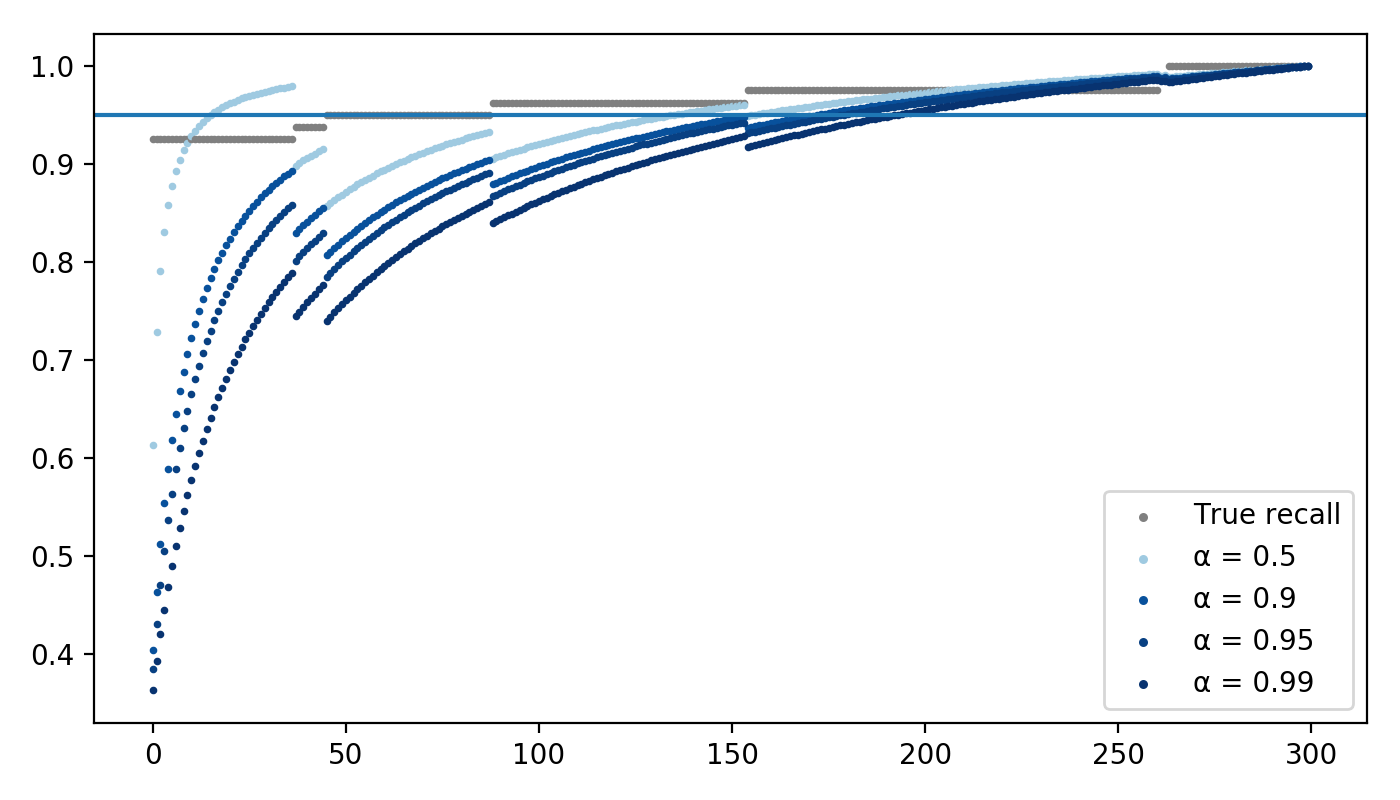
\includegraphics[width=\linewidth]{../images/sample_recall}
		\caption{Sample recall}
		\label{sample-recall}
	\end{figure}	

	\begin{figure}
		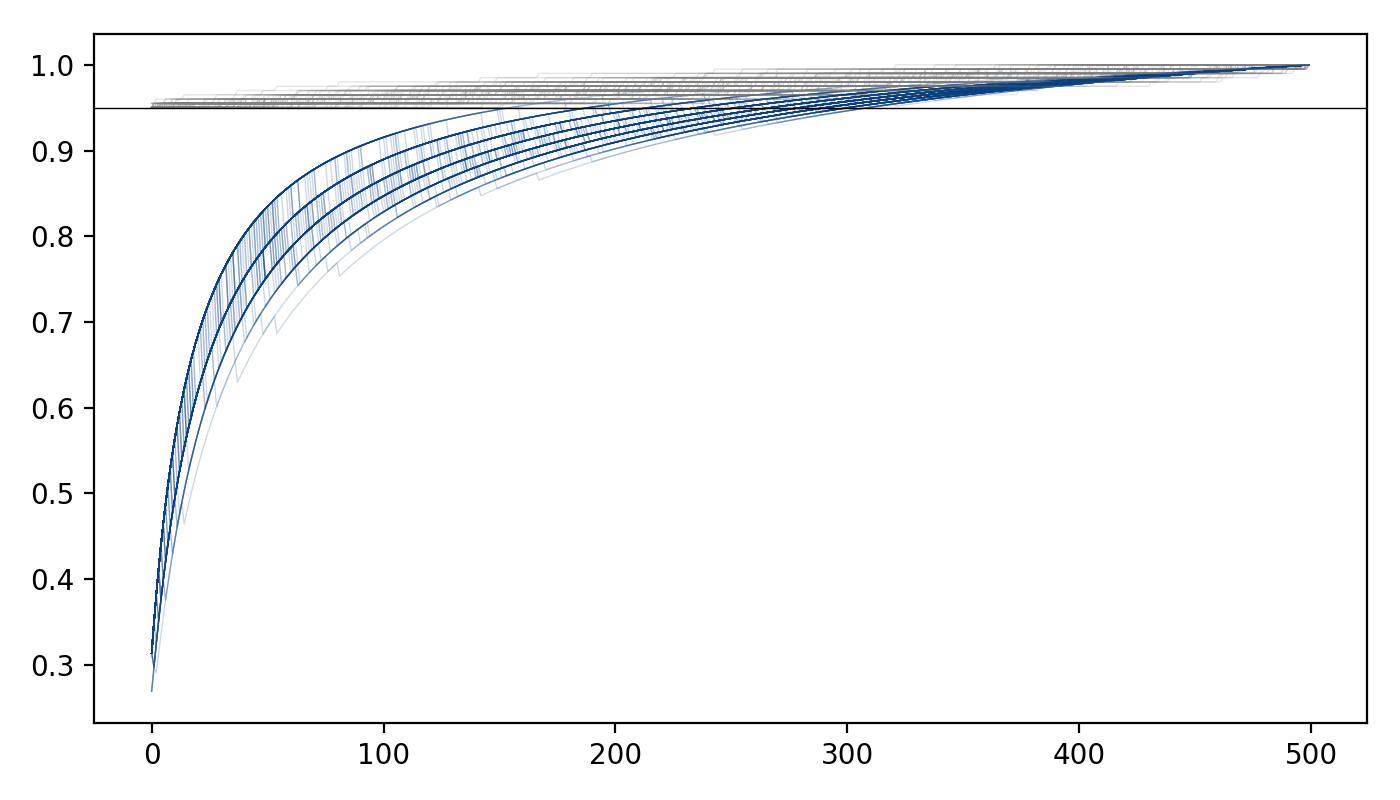
\includegraphics[width=\linewidth]{../images/sample_recall_2}
		\caption{Sample recall variation}
		\label{sample-recall-variation}
	\end{figure}	

	That the blue lines consistently meet a 95\% threshold to the right of the grey lines indicates that reviewers have to see more than 95\% of relevant documents in order to be confident that they have achieved their threshold. 
	We call the number of documents it is necessary to review to establish with confidence that reviewers have achieved 95\% recall after they have already achieved 95\% recall the \textit{additional burden}. 
	
	In figure \ref{additional-burden}, we investigate how the total number of documents and the proportion of relevant documents affect the additional burden \todo{Use the number of documents seen instead of p?}. We demonstrate the additional burden decreases \todo{how? Non-linearly?} with increasing total numbers of documents. With decreasing relevance of the remaining documents (holding the recall constant at 95\%, this means that fewer documents remain unseen), the additional burden increases. This implies that where the machine learning has more successfully identified documents and reduced burden, the additional burden required to establish the level of recall is higher. This is because the proportion of documents not seen is greater, so uncertainty around the relevance of that proportion has a greater impact on the estimation of recall.

	When to move to random sampling remains an open question. Our current approach is to use the predicted relevance of the machine learning model as a guide. We calculate the [minimum/maximum] estimated recall based on observing the predicted relevance level in [x] random documents. If the estimated recall would be below the threshold, then we begin drawing random documents.

	The stopping criteria explained here is 
	
	\subsection*{Evaluation}
	
	We evaluate each of the three criteria discussed on real world test data. With each method, we run 100 runs and record 
	\begin{itemize}
		\item \textbf{Actual Recall}: The recall when the stopping criteria is met
		\item \textbf{WS-SC}: Work saved when the stopping criteria is met \footnote{we do not use work saved over sampling, is it is not axiomatic that seeing 95\% of a random sample would achieve 95\% recall}
		\item \textbf{Additional Burden}: The proportion of the literature that need to be screened in order to \textit{be confident} that 95\% recall has been achieved, after 95\% of documents have actually been identified.
		\item \textbf{Missed Recall}: The amount by which, if any, the recall target was missed - in percentage points
	\end{itemize}
	We operationalise the heuristic stopping criteria with 50, 100, and 200 irrelevant records in a row. For simplicity, we use a basic SVM model [REFS], with 1-2 word n-grams in the document abstracts used as input data. We start with random samples of [100, 200, and 500] documents.
	
	As the intention is to evaluate stopping criteria, rather than machine learning approaches, we focus on additional burden and missed recall. These parameters correspond to the tradeoff inherent in stopping criteria: stopping too early means missing the recall target, stopping too late means undergoing additional burden than was actually required to meet the target.
	
	
	
	%\subsubsection*{Evaluation Data}
	
	We use the collection of systematic reviews used to develop machine learning applications for document screening by Aaron Cohen and co-authors in 2006 \cite{Cohen2006}, along with PB COPD, and FASTREAD \todo{fill in gaps}. We feel that testing on datasets with different properties and from different domains is key to establishing criteria appropriate for general use. In this way we can show how well the criteria perform even when the model performs badly.
	
	\section*{Results}

    \begin{figure*}
	\centering
	\begin{subfigure}[b]{0.475\textwidth}
		\centering
		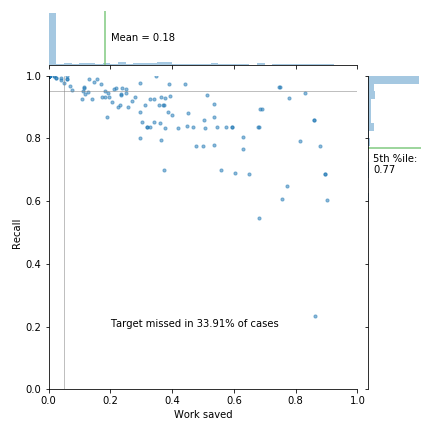
\includegraphics[width=\textwidth]{../images/jointplot_bir}
		\caption[Network2]%Example-Image
		{{\small Baseline Sampling}}    
		\label{fig:mean and std of net14}
	\end{subfigure}
	\hfill
	\begin{subfigure}[b]{0.475\textwidth}  
		\centering 
		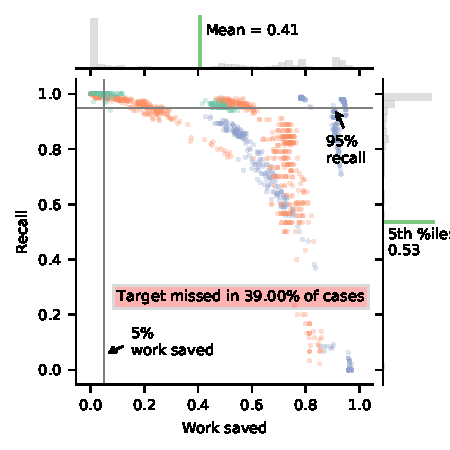
\includegraphics[width=\textwidth]{../images/jointplot_ih_50}
		\caption[]%
		{{\small 50 consecutive irrelevant results}}    
		\label{fig:mean and std of net24}
	\end{subfigure}
	\vskip\baselineskip
	\begin{subfigure}[b]{0.475\textwidth}   
		\centering 
		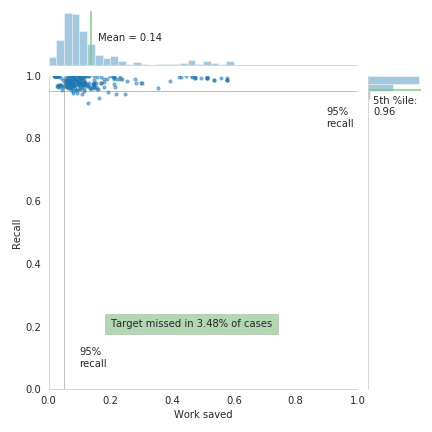
\includegraphics[width=\textwidth]{../images/jointplot_hyper}
		\caption[]%
		{{\small Hypergeometric sampling \\}}    
		\label{fig:mean and std of net34}
	\end{subfigure}
	\hfill
	\begin{subfigure}[b]{0.475\textwidth}   
		\centering 
		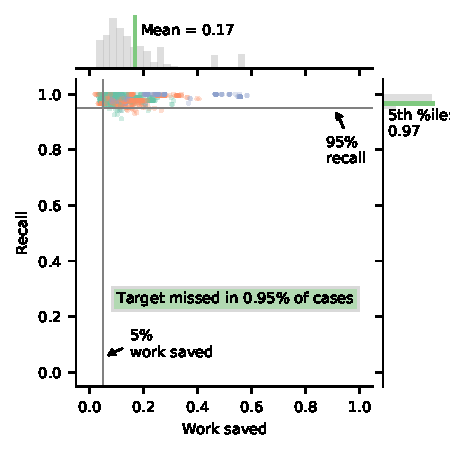
\includegraphics[width=\textwidth]{../images/jointplot_nrs}
		\caption[]%
		{{\footnotesize Pseudorandom hypergeometric sampling}}    
		\label{fig:mean and std of net44}
	\end{subfigure}
	\caption[ The average and standard deviation of critical parameters ]
	{\small The average and standard deviation of critical parameters: Region R4} 
	\label{fig:mean and std of nets}
\end{figure*}

	
	
	
	
	\section*{Discussion}
	
	\section*{Conclusion}
	
	We argue that the stopping criteria proposed here has several important advantages.
	
	\begin{itemize}
		\item The accuracy of results is independent of modelling decisions. When a model fits badly, you have to work more, but you don't miss results without knowing it.
		\item A minimum threshold with uncertainty is understandable and communicable in a live review. It is based solely on arithmetic and simple statistics.
		\item A minimum threshold better takes into account the undesirability of missed recall.
	\end{itemize}
	
\begin{backmatter}
	
	\section*{Competing interests}
	The authors declare that they have no competing interests.
	
	\section*{Author's contributions}
	Text for this section \ldots
	
	\section*{Acknowledgements}
	Max Callaghan is supported by a PhD scholarship from the Heinrich Böll Foundation
		
	\bibliography{../mendeley}
	\bibliographystyle{vancouver}
	
\end{backmatter}
\end{document}